\documentclass[tikz,border=15pt]{standalone}
\usepackage{tikz}
\usepackage{amsmath}
\usepackage{amssymb}
\usetikzlibrary{positioning, arrows.meta, calc, backgrounds, fit, shapes.geometric, decorations.pathreplacing, shadows}

% ============================================================
% COLOR DEFINITIONS
% ============================================================
\colorlet{color_intent}{blue!60!black}
\colorlet{color_slot}{green!50!black}
\colorlet{color_topic}{red!60!black}
\colorlet{color_shared}{black!70}

\begin{document}

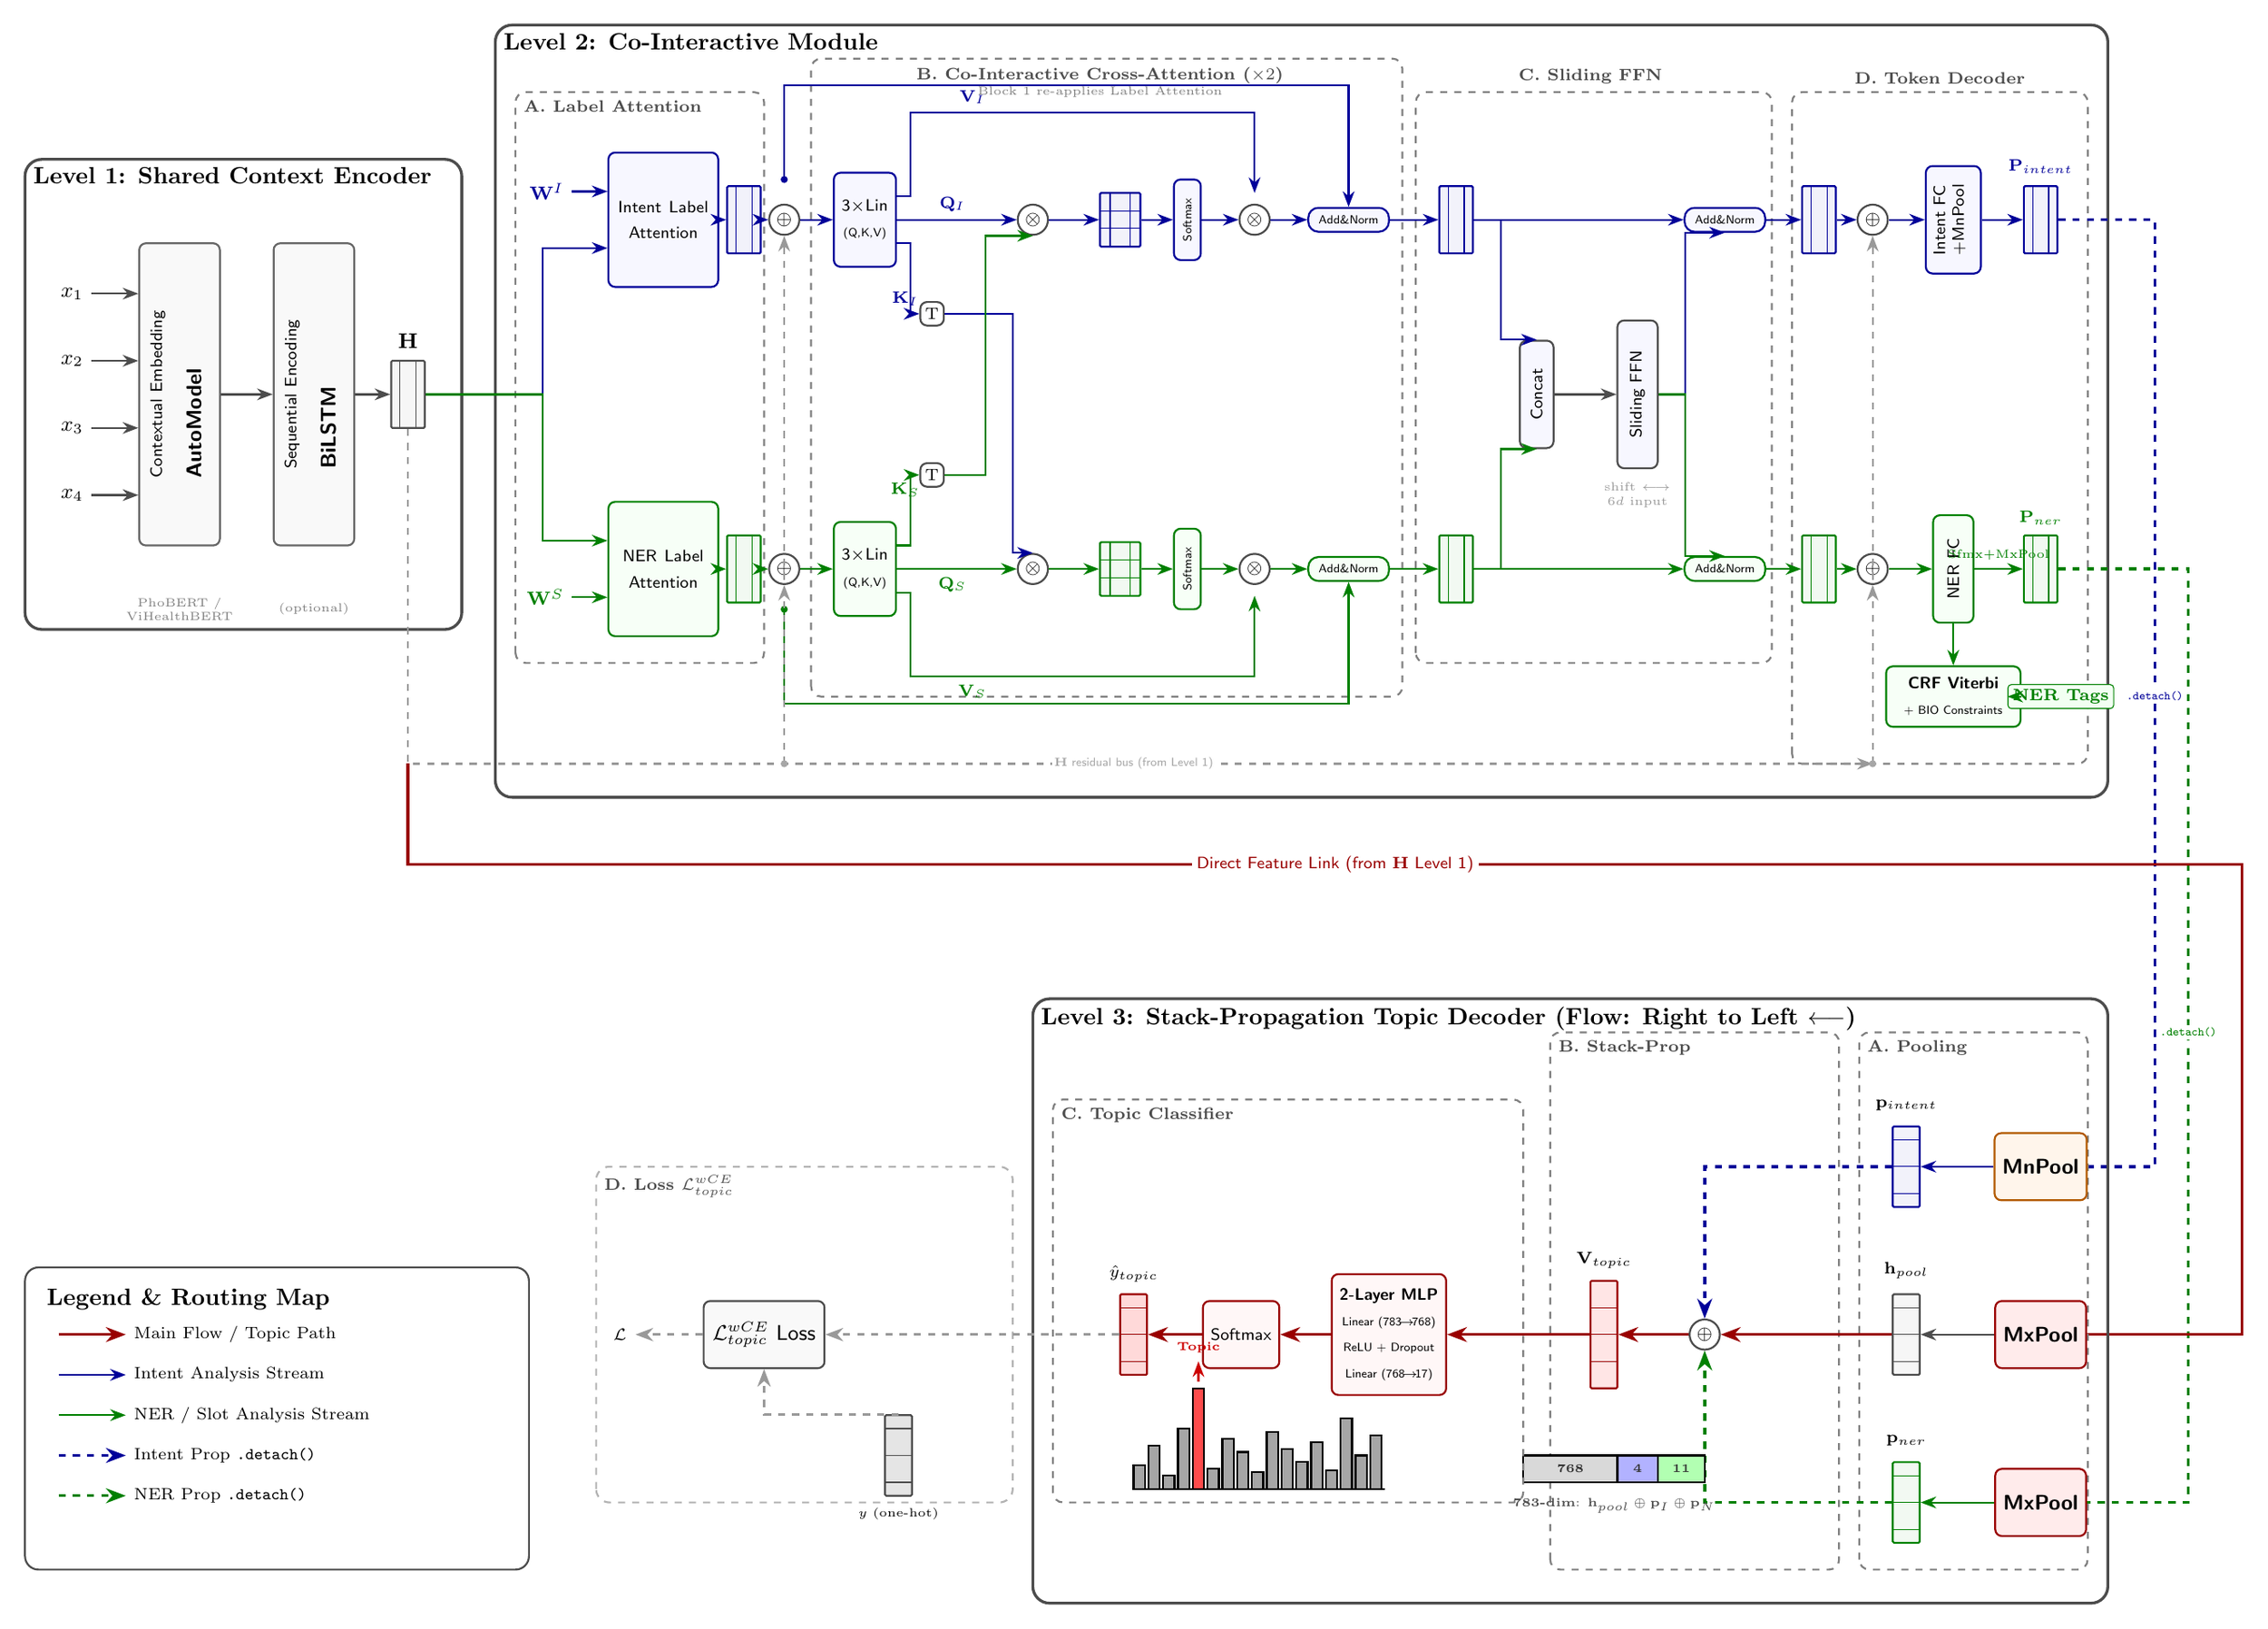
\begin{tikzpicture}[
    >=Stealth,
    font=\small\sffamily,
    color_intent/.style={blue!60!black},
    color_slot/.style={green!50!black},
    color_topic/.style={red!60!black},
    color_shared/.style={black!70},
    mainbox/.style={draw=black!70, rounded corners=2.5mm, line width=1.2pt},
    subbox/.style={draw=black!50, dashed, rounded corners=1.5mm, line width=0.8pt},
    trainbox/.style={draw=black!30, dashed, rounded corners=2mm, line width=0.8pt},
    block/.style={draw=black!70, fill=white, rounded corners=1mm, thick, align=center},
    shared_block/.style={block, draw=black!60, fill=gray!5},
    intent_block/.style={block, draw=blue!60!black, fill=blue!3},
    slot_block/.style={block, draw=green!50!black, fill=green!3},
    topic_block/.style={block, draw=red!60!black, fill=red!3},
    max_pool/.style={block, draw=red!60!black, fill=red!8, thick, minimum height=1cm},
    mean_pool/.style={block, draw=orange!70!black, fill=orange!8, thick, minimum height=1cm},
    op/.style={circle, draw=black!70, fill=white, inner sep=0.5pt, minimum size=0.45cm, thick, font=\footnotesize},
    arrow/.style={->, thick, draw=black!70},
    arrow_intent/.style={->, thick, draw=blue!60!black},
    arrow_slot/.style={->, thick, draw=green!50!black},
    link_solid/.style={->, line width=1.2pt, draw=red!60!black},
    link_dashed_blue/.style={->, line width=1.2pt, dashed, draw=blue!60!black},
    link_dashed_green/.style={->, line width=1.2pt, dashed, draw=green!50!black},
    link_dashed_gray/.style={->, line width=1.0pt, dashed, draw=gray!80},
    matrix_vert/.style={
        draw=#1, thick, fill=#1!5, minimum width=0.5cm, minimum height=1.0cm, rounded corners=0.5pt,
        path picture={
            \draw[#1, thin] (-0.12,-0.5) -- (-0.12,0.5);
            \draw[#1, thin] (0.12,-0.5) -- (0.12,0.5);
        }
    },
    matrix_grid/.style={
        draw=#1, thick, fill=#1!5, minimum width=0.6cm, minimum height=0.8cm, rounded corners=0.5pt,
        path picture={
            \draw[#1, thin] (-0.15,-0.4) -- (-0.15,0.4);
            \draw[#1, thin] (0.15,-0.4) -- (0.15,0.4);
            \draw[#1, thin] (-0.3,-0.13) -- (0.3,-0.13);
            \draw[#1, thin] (-0.3,0.13) -- (0.3,0.13);
        }
    },
    vector_grid/.style={
        draw=#1, thick, fill=#1!5, minimum width=0.4cm, minimum height=1.2cm, rounded corners=0.5pt,
        path picture={
            \foreach \y in {-0.4, 0, 0.4} \draw[#1, thin] (-0.2,\y) -- (0.2,\y);
        }
    }
]

%% ============================================================
%% TIER 1: SHARED CONTEXT ENCODER (ROW 1 - LEFT)
%% ============================================================
\draw[mainbox] (-5.5, 1.5) rectangle (1.0, 8.5);
\node[anchor=north west, font=\bfseries] at (-5.5, 8.5) {Level 1: Shared Context Encoder};

\foreach \i/\y in {1/6.5, 2/5.5, 3/4.5, 4/3.5} {
    \node (x\i) at (-4.8, \y) {$x_{\i}$};
}

\node[shared_block, minimum width=1.2cm, minimum height=4.5cm] (plm) at (-3.2, 5.0) {
    \rotatebox{90}{\scriptsize Contextual Embedding}
    \hspace{0.1cm}
    \rotatebox{90}{\textbf{AutoModel}}
};
\node[font=\tiny, text=black!50, align=center] at (-3.2, 1.8) {PhoBERT /\\ViHealthBERT};
\foreach \i in {1, 2, 3, 4} { \draw[arrow] (x\i) -- (x\i -| plm.west); }

\node[shared_block, minimum width=1.2cm, minimum height=4.5cm] (bilstm) at (-1.2, 5.0) {
    \rotatebox{90}{\scriptsize Sequential Encoding}
    \hspace{0.1cm}
    \rotatebox{90}{\textbf{BiLSTM}}
};
\node[font=\tiny, text=black!50, align=center] at (-1.2, 1.8) {(optional)};
\draw[arrow] (plm.east) -- (bilstm.west);

\node[matrix_vert=color_shared] (H_mat) at (0.2, 5.0) {};
\node[above=0.05cm of H_mat, font=\bfseries\small] {$\mathbf{H}$};
\draw[arrow] (bilstm.east) -- (H_mat.west);


%% ============================================================
%% TIER 2: CO-INTERACTIVE MODULE (ROW 1 - RIGHT)
%% ============================================================
\draw[mainbox] (1.5, -1.0) rectangle (25.5, 10.5);
\node[anchor=north west, font=\bfseries] at (1.5, 10.5) {Level 2: Co-Interactive Module};

%% --- A. LABEL ATTENTION ---
\draw[subbox] (1.8, 1.0) rectangle (5.5, 9.5);
\node[anchor=north west, font=\bfseries\scriptsize, text=black!70] at (1.8, 9.5) {A. Label Attention};

\node[intent_block, minimum height=2.0cm, text width=1.4cm] (attn_I) at (4.0, 7.6) {\scriptsize Intent Label\\Attention};
\node[slot_block, minimum height=2.0cm, text width=1.4cm] (attn_S) at (4.0, 2.4) {\scriptsize NER Label\\Attention};

\node[font=\bfseries\footnotesize, text=color_intent, anchor=east] (WI) at ([xshift=-15pt, yshift=12pt]attn_I.west) {$\mathbf{W}^I$};
\node[font=\bfseries\footnotesize, text=color_slot, anchor=east] (WS) at ([xshift=-15pt, yshift=-12pt]attn_S.west) {$\mathbf{W}^S$};

\draw[arrow_intent] (WI.east) -- ([yshift=12pt]attn_I.west);
\draw[arrow_slot] (WS.east) -- ([yshift=-12pt]attn_S.west);

\draw[arrow_intent] (H_mat.east) -- (2.2, 5.0) |- ([yshift=-12pt]attn_I.west);
\draw[arrow_slot] (H_mat.east) -- (2.2, 5.0) |- ([yshift=12pt]attn_S.west);

\node[matrix_vert=color_intent] (mat_I1) at (5.2, 7.6) {};
\node[matrix_vert=color_slot] (mat_S1) at (5.2, 2.4) {};
\draw[arrow_intent] (attn_I.east) -- (mat_I1.west);
\draw[arrow_slot] (attn_S.east) -- (mat_S1.west);

%% --- +H RESIDUAL FROM TIER 1 (before entering Cross-Attention blocks) ---
%% Code: block(H_I + H, H_N + H, mask) — label_attn output + encoder H
\node[op] (plus_blk_I) at (5.8, 7.6) {$\oplus$};
\node[op] (plus_blk_S) at (5.8, 2.4) {$\oplus$};
\draw[arrow_intent] (mat_I1.east) -- (plus_blk_I.west);
\draw[arrow_slot] (mat_S1.east) -- (plus_blk_S.west);
% H connection via bottom bus (drawn later)


%% --- B. CO-INTERACTIVE CROSS-ATTENTION (CORRECTED) ---
\draw[subbox] (6.2, 0.5) rectangle (15.0, 10.0);
\node[anchor=north, font=\bfseries\scriptsize, text=black!70] at (10.5, 10.0) {B. Co-Interactive Cross-Attention ($\times 2$)};
\node[font=\tiny, text=black!50, align=center] at (10.5, 9.5) {Block 1 re-applies Label Attention};

\node[intent_block, minimum height=1.4cm, minimum width=0.8cm] (lin_I) at (7.0, 7.6) {\scriptsize 3$\times$Lin\\\tiny(Q,K,V)};
\node[slot_block, minimum height=1.4cm, minimum width=0.8cm] (lin_S) at (7.0, 2.4) {\scriptsize 3$\times$Lin\\\tiny(Q,K,V)};
\draw[arrow_intent] (plus_blk_I.east) -- (lin_I.west);
\draw[arrow_slot] (plus_blk_S.east) -- (lin_S.west);

\node[op] (mul1_I) at (9.5, 7.6) {$\otimes$};
\node[op] (mul1_S) at (9.5, 2.4) {$\otimes$};

% Khối Transpose cho K_I và K_S
\node[block, minimum size=0.35cm, inner sep=1pt, font=\scriptsize] (T_I) at (8.0, 6.2) {T};
\node[block, minimum size=0.35cm, inner sep=1pt, font=\scriptsize] (T_S) at (8.0, 3.8) {T};

% === INTENT STREAM (MÀU XANH DƯƠNG) ===
% V_I: Đi vút lên trên cùng
\draw[arrow_intent] ([yshift=10pt]lin_I.east) -- ++(0.2,0) |- (12.8, 9.2) -- (12.8, 8.0);
\node[above, font=\scriptsize, text=color_intent] at (8.6, 9.2) {$\mathbf{V}_I$};

% Q_I: Đi thẳng
\draw[arrow_intent] (lin_I.east) -- (mul1_I.west);
\node[above, font=\scriptsize, text=color_intent] at (8.3, 7.6) {$\mathbf{Q}_I$};

% K_I: Chui vào trong, qua T_I, sau đó vòng xuống
\draw[arrow_intent] ([yshift=-10pt]lin_I.east) -- ++(0.2,0) |- (T_I.west);
\node[above, font=\scriptsize, text=color_intent] at (7.6, 6.2) {$\mathbf{K}_I$};
\draw[arrow_intent] (T_I.east) -- (9.2, 6.2) |- (mul1_S.north); % x=9.2 là làn dọc an toàn

% === SLOT STREAM (MÀU XANH LÁ) ===
% V_S: Đi tụt xuống dưới cùng
\draw[arrow_slot] ([yshift=-10pt]lin_S.east) -- ++(0.2,0) |- (12.8, 0.8) -- (12.8, 2.0);
\node[below, font=\scriptsize, text=color_slot] at (8.6, 0.8) {$\mathbf{V}_S$};

% Q_S: Đi thẳng
\draw[arrow_slot] (lin_S.east) -- (mul1_S.west);
\node[below, font=\scriptsize, text=color_slot] at (8.3, 2.4) {$\mathbf{Q}_S$};

% K_S: Chui vào trong, qua T_S, sau đó vòng lên
\draw[arrow_slot] ([yshift=10pt]lin_S.east) -- ++(0.2,0) |- (T_S.west);
\node[below, font=\scriptsize, text=color_slot] at (7.6, 3.8) {$\mathbf{K}_S$};
\draw[arrow_slot] (T_S.east) -- (8.8, 3.8) |- (mul1_I.south); % x=8.8 là làn dọc an toàn

% Phần còn lại của Module Cross-Attention
\node[matrix_grid=color_intent] (mat_I2) at (10.8, 7.6) {};
\node[intent_block, minimum height=1.2cm, minimum width=0.4cm] (soft_I) at (11.8, 7.6) {\rotatebox{90}{\tiny Softmax}};
\node[op] (mul2_I) at (12.8, 7.6) {$\otimes$};
\node[intent_block, rounded corners=1.5mm, minimum width=1.2cm] (addnorm1_I) at (14.2, 7.6) {\tiny Add\&Norm};

\node[matrix_grid=color_slot] (mat_S2) at (10.8, 2.4) {};
\node[slot_block, minimum height=1.2cm, minimum width=0.4cm] (soft_S) at (11.8, 2.4) {\rotatebox{90}{\tiny Softmax}};
\node[op] (mul2_S) at (12.8, 2.4) {$\otimes$};
\node[slot_block, rounded corners=1.5mm, minimum width=1.2cm] (addnorm1_S) at (14.2, 2.4) {\tiny Add\&Norm};

\draw[arrow_intent] (mul1_I.east) -- (mat_I2.west);
\draw[arrow_intent] (mat_I2.east) -- (soft_I.west);
\draw[arrow_intent] (soft_I.east) -- (mul2_I.west);
\draw[arrow_intent] (mul2_I.east) -- (addnorm1_I.west);
\draw[arrow_slot] (mul1_S.east) -- (mat_S2.west);
\draw[arrow_slot] (mat_S2.east) -- (soft_S.west);
\draw[arrow_slot] (soft_S.east) -- (mul2_S.west);
\draw[arrow_slot] (mul2_S.east) -- (addnorm1_S.west);

% Residual from ⊕ output (= label_attn + H) to Add&Norm
% Code: self.out_a(ctx_a, repr_a) where repr_a = block input = LA + H
\fill[color_intent] (5.8, 8.2) circle (1.5pt);
\draw[arrow_intent] (5.8, 8.2) -- (5.8, 9.6) -| (addnorm1_I.north);
\fill[color_slot] (5.8, 1.8) circle (1.5pt);
\draw[arrow_slot] (5.8, 1.8) -- (5.8, 0.4) -| (addnorm1_S.south);


%% --- C. SLIDING WINDOW FFN ---
\draw[subbox] (15.2, 1.0) rectangle (20.5, 9.5);
\node[anchor=south, font=\bfseries\scriptsize, text=black!70] at (17.8, 9.5) {C. Sliding FFN};

\node[matrix_vert=color_intent] (mat_I3) at (15.8, 7.6) {};
\node[matrix_vert=color_slot] (mat_S3) at (15.8, 2.4) {};
\draw[arrow_intent] (addnorm1_I.east) -- (mat_I3.west);
\draw[arrow_slot] (addnorm1_S.east) -- (mat_S3.west);

\node[intent_block, draw=black!70, minimum height=1.6cm, minimum width=0.5cm] (concat) at (17.0, 5.0) {\rotatebox{90}{\scriptsize Concat}};
\node[intent_block, draw=black!70, minimum height=2.2cm, minimum width=0.6cm] (ffn) at (18.5, 5.0) {\rotatebox{90}{\scriptsize Sliding FFN}};
\node[font=\tiny, text=black!40, align=center] at (18.5, 3.5) {shift $\leftarrow\!\rightarrow$\\6$d$ input};

\node[intent_block, rounded corners=1.5mm, minimum width=1.2cm] (addnorm2_I) at (19.8, 7.6) {\tiny Add\&Norm};
\node[slot_block, rounded corners=1.5mm, minimum width=1.2cm] (addnorm2_S) at (19.8, 2.4) {\tiny Add\&Norm};

\draw[arrow_intent] (mat_I3.east) -- (addnorm2_I.west);
\draw[arrow_slot] (mat_S3.east) -- (addnorm2_S.west);
\draw[arrow_intent] (mat_I3.east) -- ++(0.4, 0) |- (concat.north);
\draw[arrow_slot] (mat_S3.east) -- ++(0.4, 0) |- (concat.south);
\draw[arrow] (concat.east) -- (ffn.west);
\draw[arrow_intent] (ffn.east) -- ++(0.4, 0) |- (addnorm2_I.south);
\draw[arrow_slot] (ffn.east) -- ++(0.4, 0) |- (addnorm2_S.north);


%% --- D. TOKEN DECODER (CORRECTED: +H skip connection before FC) ---
\draw[subbox] (20.8, -0.5) rectangle (25.2, 9.5);
\node[anchor=south, font=\bfseries\scriptsize, text=black!70] at (23.0, 9.5) {D. Token Decoder};

\node[matrix_vert=color_intent] (mat_out_I) at (21.2, 7.6) {};
\node[matrix_vert=color_slot] (mat_out_S) at (21.2, 2.4) {};
\draw[arrow_intent] (addnorm2_I.east) -- (mat_out_I.west);
\draw[arrow_slot] (addnorm2_S.east) -- (mat_out_S.west);

% +H before FC heads: code does intent_fc(H_I + H) and ner_fc(H_N + H)
\node[op] (plus_dec_I) at (22.0, 7.6) {$\oplus$};
\node[op] (plus_dec_S) at (22.0, 2.4) {$\oplus$};
\draw[arrow_intent] (mat_out_I.east) -- (plus_dec_I.west);
\draw[arrow_slot] (mat_out_S.east) -- (plus_dec_S.west);
% H connection via bottom bus (drawn later)

\node[intent_block, minimum height=1.6cm, minimum width=0.6cm, align=center] (dec_I) at (23.2, 7.6) {
    \rotatebox{90}{\scriptsize Intent FC}
    \rotatebox{90}{\scriptsize +MnPool}
};
\draw[arrow_intent] (plus_dec_I.east) -- (dec_I.west);
\node[matrix_vert=color_intent] (P_I) at (24.5, 7.6) {};
\node[above=0.05cm of P_I, font=\bfseries\scriptsize, text=color_intent] {$\mathbf{P}_{intent}$};
\draw[arrow_intent] (dec_I.east) -- (P_I.west);

\node[slot_block, minimum height=1.6cm, minimum width=0.6cm, align=center] (dec_S) at (23.2, 2.4) {\rotatebox{90}{\scriptsize NER FC}};
\draw[arrow_slot] (plus_dec_S.east) -- (dec_S.west);

\node[matrix_vert=color_slot] (P_S) at (24.5, 2.4) {};
\node[above=0.02cm of P_S, font=\bfseries\scriptsize, text=color_slot] {$\mathbf{P}_{ner}$};
\draw[arrow_slot] (dec_S.east) -- (P_S.west) node[midway, above, font=\tiny, text=color_slot] {Sfmx+MxPool};

\node[slot_block, minimum height=0.9cm, minimum width=2.0cm, align=center] (crf_block) at (23.2, 0.5) {
    \scriptsize \textbf{CRF Viterbi}\\
    \tiny + BIO Constraints
};
\draw[arrow_slot] (dec_S.south) -- (crf_block.north);
\node[font=\scriptsize\bfseries, text=color_slot, fill=green!5, draw=green!50!black,
      rounded corners=0.5mm, inner sep=2pt] (ner_tags_out) at (24.8, 0.5) {NER Tags};
\draw[arrow_slot] (crf_block.east) -- (ner_tags_out.west);


%% ============================================================
%% H DISTRIBUTION BUS (connects to ⊕ nodes in Tier 2 + Tier 3)
%% ============================================================
%% Code: block(H_I + H, ...) and intent_fc(H_I + H)
%% H feeds into 4 ⊕ nodes: 2 before cross-attn blocks, 2 before FC decoders

% H bus: runs along bottom of Tier 2 at y=-0.5
\draw[link_dashed_gray, line width=0.8pt] (H_mat.south) -- (0.2, -0.5) -- (22.0, -0.5);
\node[font=\tiny\sffamily, text=gray!70, fill=white, inner sep=1pt] at (11.0, -0.5) {$\mathbf{H}$ residual bus (from Level 1)};

% Branch to ⊕ before cross-attention blocks
\draw[link_dashed_gray, line width=0.8pt] (5.8, -0.5) -- (plus_blk_I.south);
\draw[link_dashed_gray, line width=0.8pt] (5.8, -0.5) -- (plus_blk_S.south);
\fill[gray!70] (5.8, -0.5) circle (1.5pt);

% Branch to ⊕ before FC decoder heads
\draw[link_dashed_gray, line width=0.8pt] (22.0, -0.5) -- (plus_dec_I.south);
\draw[link_dashed_gray, line width=0.8pt] (22.0, -0.5) -- (plus_dec_S.south);
\fill[gray!70] (22.0, -0.5) circle (1.5pt);

%% ============================================================
%% PROPAGATION LINKS (Tier 2 → Tier 3)
%% ============================================================
% P_I drops to Tier 3
\draw[link_dashed_blue] (P_I.east) -- (26.2, 7.6) |- (24.5, -6.5);
\node[font=\tiny\ttfamily, text=blue!60!black, fill=white, inner sep=1pt] at (26.2, 0.5) {.detach()};

% P_S drops to Tier 3
\draw[link_dashed_green] (P_S.east) -- (26.7, 2.4) |- (24.5, -11.5);
\node[font=\tiny\ttfamily, text=green!50!black, fill=white, inner sep=1pt] at (26.7, -4.5) {.detach()};

% H_mat drops to Tier 3 (topic pooling)
\draw[link_solid] (0.2, -0.5) -- (0.2, -2.0) -- (27.5, -2.0) |- (24.5, -9.0);
\node[font=\scriptsize\sffamily, text=color_topic, fill=white, inner sep=2pt] at (14.0, -2.0) {Direct Feature Link (from $\mathbf{H}$ Level 1)};


%% ============================================================
%% TIER 3: STACK-PROPAGATION TOPIC DECODER (ROW 2 - R->L FLOW)
%% ============================================================
\draw[mainbox] (9.5, -13.0) rectangle (25.5, -4.0);
\node[anchor=north west, font=\bfseries] at (9.5, -4.0) {Level 3: Stack-Propagation Topic Decoder (Flow: Right to Left $\longleftarrow$)};

%% --- A. Sentence-level Pooling ---
\draw[subbox] (21.8, -12.5) rectangle (25.2, -4.5);
\node[anchor=north west, font=\bfseries\scriptsize, text=black!70] at (21.8, -4.5) {A. Pooling};

\node[mean_pool] (l3_pool_I) at (24.5, -6.5) {\textbf{MnPool}};
\node[vector_grid=color_intent] (l3_vec_I) at (22.5, -6.5) {};
\node[above=0.1cm of l3_vec_I, font=\scriptsize] {$\mathbf{p}_{intent}$};
\draw[arrow_intent] (l3_pool_I.west) -- (l3_vec_I.east);

\node[max_pool] (l3_pool_H) at (24.5, -9.0) {\textbf{MxPool}};
\node[vector_grid=color_shared] (l3_vec_H) at (22.5, -9.0) {};
\node[above=0.1cm of l3_vec_H, font=\scriptsize] {$\mathbf{h}_{pool}$};
\draw[arrow] (l3_pool_H.west) -- (l3_vec_H.east);

\node[max_pool] (l3_pool_S) at (24.5, -11.5) {\textbf{MxPool}};
\node[vector_grid=color_slot] (l3_vec_S) at (22.5, -11.5) {};
\node[above=0.1cm of l3_vec_S, font=\scriptsize] {$\mathbf{p}_{ner}$};
\draw[arrow_slot] (l3_pool_S.west) -- (l3_vec_S.east);

%% --- B. Stack-Propagation ---
\draw[subbox] (17.2, -12.5) rectangle (21.5, -4.5);
\node[anchor=north west, font=\bfseries\scriptsize, text=black!70] at (17.2, -4.5) {B. Stack-Prop};

\node[op] (l3_concat) at (19.5, -9.0) {$\oplus$};
\node[vector_grid=color_topic, fill=red!10, minimum height=1.6cm] (l3_vec_V) at (18.0, -9.0) {};
\node[above=0.05cm of l3_vec_V, font=\scriptsize] {$\mathbf{V}_{topic}$};

\draw[link_dashed_blue] (l3_vec_I.west) -| (19.5, -6.5) -- (l3_concat.north);
\draw[link_solid] (l3_vec_H.west) -- (l3_concat.east);
\draw[link_dashed_green] (l3_vec_S.west) -| (19.5, -11.5) -- (l3_concat.south);
\draw[link_solid] (l3_concat.west) -- (l3_vec_V.east);

% 783-dim bar: order matches code — cat([h_pool, intent, ner])
\begin{scope}[shift={(18.0, -11.0)}]
    \draw[fill=gray!30, thick] (-1.2, -0.2) rectangle (0.2, 0.2);
    \node[font=\tiny, text=black!80] at (-0.5, 0) {\textbf{768}};
    \draw[fill=blue!30, thick] (0.2, -0.2) rectangle (0.8, 0.2);
    \node[font=\tiny, text=black!80] at (0.5, 0) {\textbf{4}};
    \draw[fill=green!30, thick] (0.8, -0.2) rectangle (1.5, 0.2);
    \node[font=\tiny, text=black!80] at (1.15, 0) {\textbf{11}};
    \node[font=\tiny, align=center, text=black!70] at (0.15, -0.55)
        {\textbf{783-dim}: $\mathbf{h}_{pool} \oplus \mathbf{p}_I \oplus \mathbf{p}_N$};
\end{scope}

%% --- C. 2-Layer MLP Topic Classifier ---
\draw[subbox] (9.8, -11.5) rectangle (16.8, -5.5);
\node[anchor=north west, font=\bfseries\scriptsize, text=black!70] at (9.8, -5.5) {C. Topic Classifier};

\node[topic_block, minimum width=1.7cm, minimum height=1.8cm, align=center] (l3_lin_topic) at (14.8, -9.0) {
    \scriptsize \textbf{2-Layer MLP}\\
    \tiny Linear (783$\!\to\!$768)\\
    \tiny ReLU + Dropout\\
    \tiny Linear (768$\!\to\!$17)
};
\node[topic_block, minimum width=0.8cm, minimum height=1.0cm] (l3_soft_topic) at (12.6, -9.0) {\scriptsize Softmax};
\node[vector_grid=color_topic, fill=red!15] (l3_yhat) at (11.0, -9.0) {};
\node[above=0.05cm of l3_yhat, font=\scriptsize] {$\hat{y}_{topic}$};

\draw[link_solid] (l3_vec_V.west) -- (l3_lin_topic.east);
\draw[link_solid] (l3_lin_topic.west) -- (l3_soft_topic.east);
\draw[link_solid] (l3_soft_topic.west) -- (l3_yhat.east);

\begin{scope}[shift={(11.0, -11.3)}]
    \foreach \i/\h in {
        1/0.35, 2/0.65, 3/0.20, 4/0.90,
        5/1.50,
        6/0.30, 7/0.75, 8/0.55, 9/0.25,
        10/0.85, 11/0.60, 12/0.40, 13/0.70,
        14/0.28, 15/1.05, 16/0.50, 17/0.80
    } {
        \draw[fill=black!35, thick] (\i*0.22-0.22, 0) rectangle ++(0.17, \h);
    }
    \draw[fill=red!70, thick] (5*0.22-0.22, 0) rectangle ++(0.17, 1.50);
    \draw[->, thick, red!80!black] (5*0.22-0.135, 1.6) -- ++(0, 0.3)
        node[above, font=\tiny\bfseries, text=red!80!black] {Topic};
    \draw[thick] (0, 0) -- (17*0.22, 0);
\end{scope}

%% ============================================================
%% D. TRAINING: Weighted Cross-Entropy Loss
%% ============================================================
\draw[trainbox] (3.0, -11.5) rectangle (9.2, -6.5);
\node[anchor=north west, font=\bfseries\scriptsize, text=black!70] at (3.0, -6.5)
    {D. Loss $\mathcal{L}_{topic}^{wCE}$};

\node[block, minimum width=1.8cm, minimum height=1.0cm, fill=gray!5] (l3_loss) at (5.5, -9.0)
    {$\mathcal{L}_{topic}^{wCE}$ Loss};
\node[vector_grid=color_shared, fill=gray!20] (l3_y_true) at (7.5, -10.8) {};
\node[below=0.05cm of l3_y_true, font=\tiny] {$y$ (one-hot)};

\draw[link_dashed_gray] (l3_yhat.west) -- (l3_loss.east);
\draw[link_dashed_gray] (l3_y_true.north) -| (l3_loss.south);
\draw[link_dashed_gray] (l3_loss.west) -- ++(-1.0, 0) node[left, font=\bfseries\scriptsize] {$\mathcal{L}$};


%% ============================================================
%% LEGEND
%% ============================================================
\draw[draw=black!70, rounded corners=2mm, fill=white, thick] (-5.5, -12.5) rectangle (2.0, -8.0);
\node[font=\bfseries, anchor=north west] at (-5.3, -8.2) {Legend \& Routing Map};

\draw[link_solid] (-5.0, -9.0) -- (-4.0, -9.0);
\node[anchor=west, font=\scriptsize] at (-4.0, -9.0) {Main Flow / Topic Path};

\draw[arrow_intent] (-5.0, -9.6) -- (-4.0, -9.6);
\node[anchor=west, font=\scriptsize] at (-4.0, -9.6) {Intent Analysis Stream};

\draw[arrow_slot] (-5.0, -10.2) -- (-4.0, -10.2);
\node[anchor=west, font=\scriptsize] at (-4.0, -10.2) {NER / Slot Analysis Stream};

\draw[link_dashed_blue] (-5.0, -10.8) -- (-4.0, -10.8);
\node[anchor=west, font=\scriptsize] at (-4.0, -10.8)
    {Intent Prop \texttt{.detach()}};

\draw[link_dashed_green] (-5.0, -11.4) -- (-4.0, -11.4);
\node[anchor=west, font=\scriptsize] at (-4.0, -11.4)
    {NER Prop \texttt{.detach()}};

\end{tikzpicture}

\end{document}